%%%%%%%%%%%%%%%%%%%%%%%%%%%%%%%%%%%%%%%%%
% Cleese Assignment (For Students)
% LaTeX Template
% Version 2.0 (27/5/2018)
%
% This template originates from:
% http://www.LaTeXTemplates.com
%
% Author:
% Vel (vel@LaTeXTemplates.com)
%
% License:
% CC BY-NC-SA 3.0 (http://creativecommons.org/licenses/by-nc-sa/3.0/)
% 
%%%%%%%%%%%%%%%%%%%%%%%%%%%%%%%%%%%%%%%%%

%----------------------------------------------------------------------------------------
%	PACKAGES AND OTHER DOCUMENT CONFIGURATIONS
%----------------------------------------------------------------------------------------

\documentclass[10pt]{article}
% %%%%%%%%%%%%%%%%%%%%%%%%%%%%%%%%%%%%%%%%%
% Cleese Assignment
% Structure Specification File
% Version 1.0 (27/5/2018)
%
% This template originates from:
% http://www.LaTeXTemplates.com
%
% Author:
% Vel (vel@LaTeXTemplates.com)
%
% License:
% CC BY-NC-SA 3.0 (http://creativecommons.org/licenses/by-nc-sa/3.0/)
% 
%%%%%%%%%%%%%%%%%%%%%%%%%%%%%%%%%%%%%%%%%

%----------------------------------------------------------------------------------------
%	PACKAGES AND OTHER DOCUMENT CONFIGURATIONS
%----------------------------------------------------------------------------------------

\usepackage{lastpage} % Required to determine the last page number for the footer

\usepackage{graphicx} % Required to insert images

\setlength\parindent{0pt} % Removes all indentation from paragraphs

\usepackage[svgnames]{xcolor} % Enabling colors by their 'svgnames'
\usepackage[most]{tcolorbox} % Required for boxes that split across pages

\usepackage{booktabs} % Required for better horizontal rules in tables

\usepackage{listings} % Required for insertion of code

\usepackage{etoolbox} % Required for if statements

\usepackage{multido} % required for dotted lines

\usepackage[french]{babel} % English language hyphenation

\usepackage{svg}

%----------------------------------------------------------------------------------------
%	MARGINS
%----------------------------------------------------------------------------------------

\usepackage{geometry} % Required for adjusting page dimensions and margins

\geometry{
	paper=a4paper, % Change to letterpaper for US letter
	top=3cm, % Top margin
	bottom=3cm, % Bottom margin
	left=2.5cm, % Left margin
	right=2.5cm, % Right margin
	headheight=14pt, % Header height
	footskip=1.4cm, % Space from the bottom margin to the baseline of the footer
	headsep=1.2cm, % Space from the top margin to the baseline of the header
	%showframe, % Uncomment to show how the type block is set on the page
}

%----------------------------------------------------------------------------------------
%	FONT
%----------------------------------------------------------------------------------------
\usepackage{fontspec}
\usepackage{unicode-math}
\usepackage[utf8]{inputenc} % Required for inputting international characters
\usepackage[T1]{fontenc} % Output font encoding for international characters

\setmainfont[Ligatures=TeX]{Caladea}
%----------------------------------------------------------------------------------------
%	HEADERS AND FOOTERS
%----------------------------------------------------------------------------------------

\usepackage{fancyhdr} % Required for customising headers and footers

\pagestyle{fancy} % Enable custom headers and footers

% \lhead{\small\assignmentClass\ifdef{\assignmentClassInstructor}{\ (\assignmentClassInstructor):}{}\ \assignmentTitle} % Left header; output the instructor in brackets if one was set
% \chead{} % Centre header
% \rhead{\small\ifdef{\assignmentAuthorName}{\assignmentAuthorName}{\ifdef{\assignmentDueDate}{Due\ \assignmentDueDate}{}}} % Right header; output the author name if one was set, otherwise the due date if that was set

% \lfoot{} % Left footer
% \cfoot{\small Page\ \thepage\ sur\ \pageref{LastPage}} % Centre footer
% \rfoot{} % Right footer

% \renewcommand\headrulewidth{0.5pt} % Thickness of the header rule


% \fancypagestyle{plain}{
% 	\lhead{} % Left header; output the instructor in brackets if one was set
% 	\chead{} % Centre header
% 	\rhead{}

%   \renewcommand{\headrulewidth}{0pt}%
%   \fancyfoot[C]{\small Page\ \thepage\ sur\ \pageref{LastPage}}%
% }

%----------------------------------------------------------------------------------------
%	MODIFY SECTION STYLES
%----------------------------------------------------------------------------------------

% \usepackage{titlesec} % Required for modifying sections

%------------------------------------------------
% Section

% \titleformat
% {\section} % Section type being modified
% [block] % Shape type, can be: hang, block, display, runin, leftmargin, rightmargin, drop, wrap, frame
% {\Large\bfseries} % Format of the whole section
% {\assignmentQuestionName~\thesection} % Format of the section label
% {6pt} % Space between the title and label
% {} % Code before the label

% \titlespacing{\section}{0pt}{0.5\baselineskip}{0.5\baselineskip} % Spacing around section titles, the order is: left, before and after

%------------------------------------------------
% Subsection

% \titleformat
% {\subsection} % Section type being modified
% [block] % Shape type, can be: hang, block, display, runin, leftmargin, rightmargin, drop, wrap, frame
% {\itshape} % Format of the whole section
% {(\alph{subsection})} % Format of the section label
% {4pt} % Space between the title and label
% {} % Code before the label

% \titlespacing{\subsection}{0pt}{0.5\baselineskip}{0.5\baselineskip} % Spacing around section titles, the order is: left, before and after

% \renewcommand\thesubsection{(\alph{subsection})}

%----------------------------------------------------------------------------------------
%	CUSTOM QUESTION COMMANDS/ENVIRONMENTS
%----------------------------------------------------------------------------------------


%	TITLE SECTION
%----------------------------------------------------------------------------------------

% \newcommand{\authorstyle}[1]{{\large\usefont{OT1}{phv}{b}{n}#1}} % Authors style (Helvetica)

% \newcommand{\institution}[1]{{\footnotesize\usefont{OT1}{phv}{m}{sl}#1}} % Institutions style (Helvetica)

% \usepackage{titling} % Allows custom title configuration

% \newcommand{\HorRule}{\rule{\linewidth}{1pt}} % Defines the gold horizontal rule around the title

% \pretitle{
% 	\centering
% 	\vspace{-120pt} % Move the entire title section up
% 	\HorRule\vspace{10pt} % Horizontal rule before the title
% 	% \textbf
% 	\bfseries
% 	\fontsize{32}{36}
% 	\usefont{T1}{phv}{b}{n}
% 	\selectfont % Helvetica
% 	\color{DarkRed} % Text colour for the title and author(s)
% }

% \posttitle{\par\vskip 15pt} % Whitespace under the title

% \preauthor{} % Anything that will appear before \author is printed

% \postauthor{ % Anything that will appear after \author is printed
% 	% \vspace{10pt} % Space before the rule
% 	\par\HorRule % Horizontal rule after the title
% 	\vspace{-30pt} % Space after the title section
% }

 % Include the file specifying the document structure and custom commands
\input{/home/astrale/Cours/EDUCATION_NATIONALE/mes_cours/2121-22/templates/activité/act/activite.sty} % Include the file specifying the document structure and custom commands


%----------------------------------------------------------------------------------------
%	ASSIGNMENT INFORMATION
%----------------------------------------------------------------------------------------

% Required
\newcommand{\assignmentQuestionName}{Question} % The word to be used as a prefix to question numbers; example alternatives: Problem, Exercise
\newcommand{\assignmentClass}{Physique Chimie} % Course/class
\newcommand{\assignmentTitle}{Activité n°2} % Assignment title or name
\newcommand{\assignmentAuthorName}{Chapitre 3} %

%----------------------------------------------------------------------------------------
%	VARIABLES
%----------------------------------------------------------------------------------------

\newcommand{\titreActivite}{
	\huge Activité 2: Différence entre 
	circuits en série et circuits en dérivation.} % titre de l'activité
\newcommand{\objectif}{ 	
	\begin{itemize}
		\item Connaître l'influence du nombre de dipôle, 
		l'ordre des dipôles et d'une panne de dipôle sur 
		un circuit en série ou en dérivation.
	\end{itemize}
} % titre de l'activité
\newcommand{\contexte}{ 
	}
\newcommand{\resumeContexte}{

	} 





%----------------------------------------------------------------------------------------

\begin{document}
%----------------------------------------------------------------------------------------
%	TITLE PAGE
%----------------------------------------------------------------------------------------
\date{}
\title{\titreActivite}
\maketitle % Print the title page

\underline{\textbf{Objectif}} :  \vspace{2pt}
\objectif

\vspace{8pt}

% \underline{\textbf{Contexte}} :  \textit{\contexte}

\begin{center}
	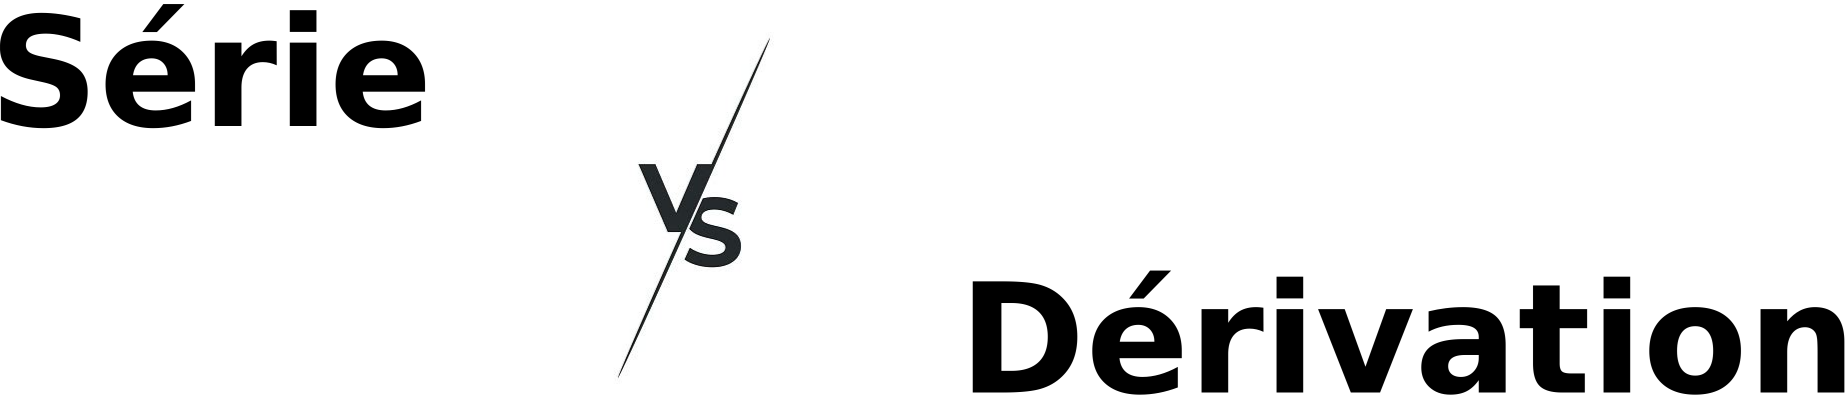
\includegraphics[width=0.4\columnwidth]{vs.png} % Example image
\end{center}

\textbf{\resumeContexte}
\vspace{-12pt}
%% ----------------------------------

\assignmentSection{Votre mission travail}

%----------------------------------------------------------------------------------------
%	QUESTION 
%----------------------------------------------------------------------------------------

\begin{question}
	\questiontext{
		Pour chacune des tables suivantes:
	}
	\end{question}
	
	\subquestion{\textbf{Réaliser} les circuits représentés.}
	\subquestion{\textbf{Compléter} les phrases de conclusion sur les pointillés.}
%	\answerbox{}
% \setlength{\arrayrulewidth}{0.5mm}
% \setlength{\tabcolsep}{18pt}

\renewcommand{\arraystretch}{1.5}
% \begin{center}
	\centering
	\begin{tabular}{cc} \toprule
		\multicolumn{2}{c}{Influence du nombre de recepteur} \\ \midrule
		% \cmidrule{1-2}
		Circuit en série & Circuit en dérivation\\ \midrule
		\includegraphics[width=0.23\columnwidth]{nb_dipole1.png} 
								& \includegraphics[width=0.23\columnwidth]{nb_dipole2.png} \\
		% 
		\parbox[t]{0.47\textwidth}{
		Plus le nombre de récepteurs
					est important, plus
					\answerbox{1}
					} 			& \parbox[t]{0.47\textwidth}{
								Plus le nombre de récepteurs
								est important, plus
								\answerbox{1} }
													\\ %\bottomrule
	\end{tabular}
	\begin{tabular}{cc} \toprule
		\multicolumn{2}{c}{Influence de l'ordre des dipôles} \\ \midrule
		% \cmidrule{1-2}
		Circuit en série & Circuit en dérivation\\ \midrule
		\includegraphics[width=0.3\columnwidth]{ordre_dipole1.png} 
								& \includegraphics[width=0.2\columnwidth]{ordre_dipole2.png} \\
		% 
		\parbox[t]{0.47\textwidth}{
			Quand on change l'ordre des dipôle,
			on observe
			\answerbox{1}}
								& \parbox[t]{0.47\textwidth}{
									Quand on change l'ordre des dipôle,
									on observe \answerbox{1}
									} \\
	\end{tabular}
% \end{center}

% \begin{center}
	\begin{tabular}{cc} \toprule
		\multicolumn{2}{c}{Influence d'une lampe dévissée ou grillé.} \\ \midrule
		% \cmidrule{1-2}
		Circuit en série & Circuit en dérivation\\ \midrule
		\includegraphics[width=0.2\columnwidth]{disfonctionne1.png} 
								& \includegraphics[width=0.12\columnwidth]{disfonctionne2.png} \\
		% 
		\parbox[t]{0.47\textwidth}{
			Si une lampe est dévissée ou grillée, le circuit \vspace{10pt}\answerbox{2}}
								& \parbox[t]{0.47\textwidth}{
									Si une lampe est dévissée ou grillée, le circuit \vspace{10pt}\answerbox{2}
									} \\
	\end{tabular}
% \end{center}


% \begin{center}
	\begin{tabular}{cc} \toprule
		\multicolumn{2}{c}{Influence d'un court circuit} \\ \midrule
		% \cmidrule{1-2}
		Circuit en série & Circuit en dérivation\\ \midrule
		\includegraphics[width=0.45\columnwidth]{court_circuit1.png} 
								& \includegraphics[width=0.2\columnwidth]{court_circuit2.png} \\
		% 
		\parbox[t]{0.47\textwidth}{
			\begin{itemize}
				\item Si la lampe OU le moteur est court circuité alors
			\end{itemize}
			\answerbox{2}
			\begin{itemize}
				\item Si la pile est court circuité alors 
			\end{itemize}
			\answerbox{1}
			\begin{itemize}
				\item On peut dire si le circuit est dangereux (ou pas) car
			\end{itemize}
			\answerbox{2}
			}
								& \parbox[t]{0.47\textwidth}{
									\begin{itemize}
										\item Si la lampe OU le moteur est court circuitée alors
									\end{itemize}
									\answerbox{2}
									\begin{itemize}
										\item Si la pile est court circuitée alors 
									\end{itemize}
									\answerbox{1}
									\begin{itemize}
										\item On peut dire si le circuit est dangereux (ou pas) car
									\end{itemize}
									\answerbox{2}
									} \\
	\end{tabular}
% \end{center}

\end{document}
